\begin{figure}
	\centering
	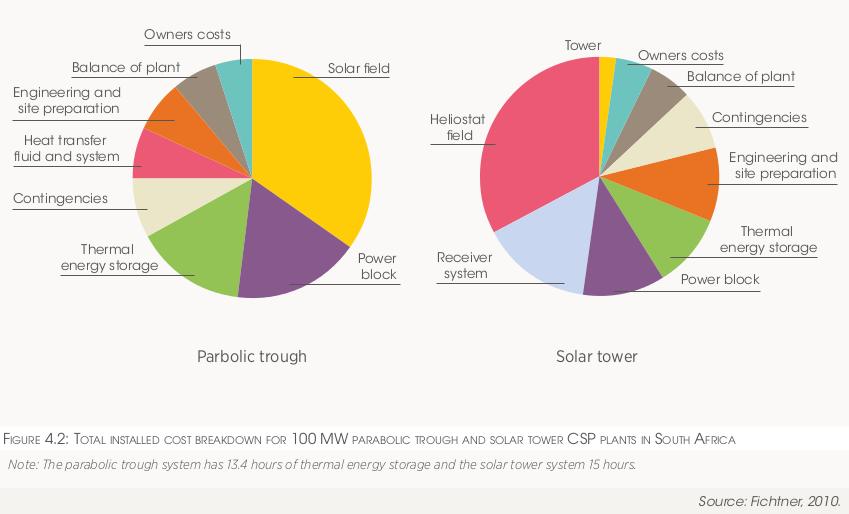
\includegraphics[width=0.9\textwidth]{kostenverteilung.png}
	\caption{Kostenverteilung CSP-Kraftwerke}
	\label{fig:kostenverteilung}
\end{figure}

Der größte Anteil der Kosten eines CSP-Kraftwerks liegt in der initialen Investition bei etwa 80\,\% der Gesamtkosten~\cite{irena2012}. Der Rest der Kosten verteilt sich auf Betrieb und Wartung sowie Versicherung des Kraftwerks.

Die IRENA schätzt die Investitionskosten auf derzeit 4500 - 7150 USD/kWh für ein Solarthermiekraftwerk ohne Wärmespeicher und auf 5000 - 10500 USD/kWh für solche mit Wärmespeicher.

Eine genauere Aufschlüsselung der Investitionskosten zeigt Abbildung~\ref{fig:kostenverteilung}. Der größte Anteil bei Parabolrinnenkraftwerken fällt dabei auf das "`Solar Field"', also den Reflektor-Teil des Kraftwerks. Bei Kraftwerken mit mehr thermischem Speicher sinkt dieser relative Anteil, weil die Speicherkomponente ebenfalls einen erheblichen Teil ausmacht.

\subsection{Zukünftige Entwicklung}

\begin{figure}
	\centering
	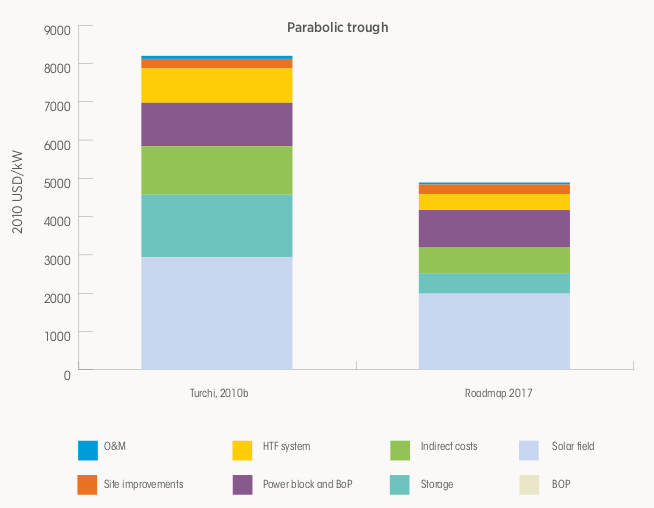
\includegraphics[width=0.9\textwidth]{kostenentwicklung1.png}
	\caption{Voraussichtliche Kostenentwicklung laut IEA CSP-Roadmap 2010}
	\label{fig:kostenentwicklung1}
\end{figure}

\begin{figure}
	\centering
	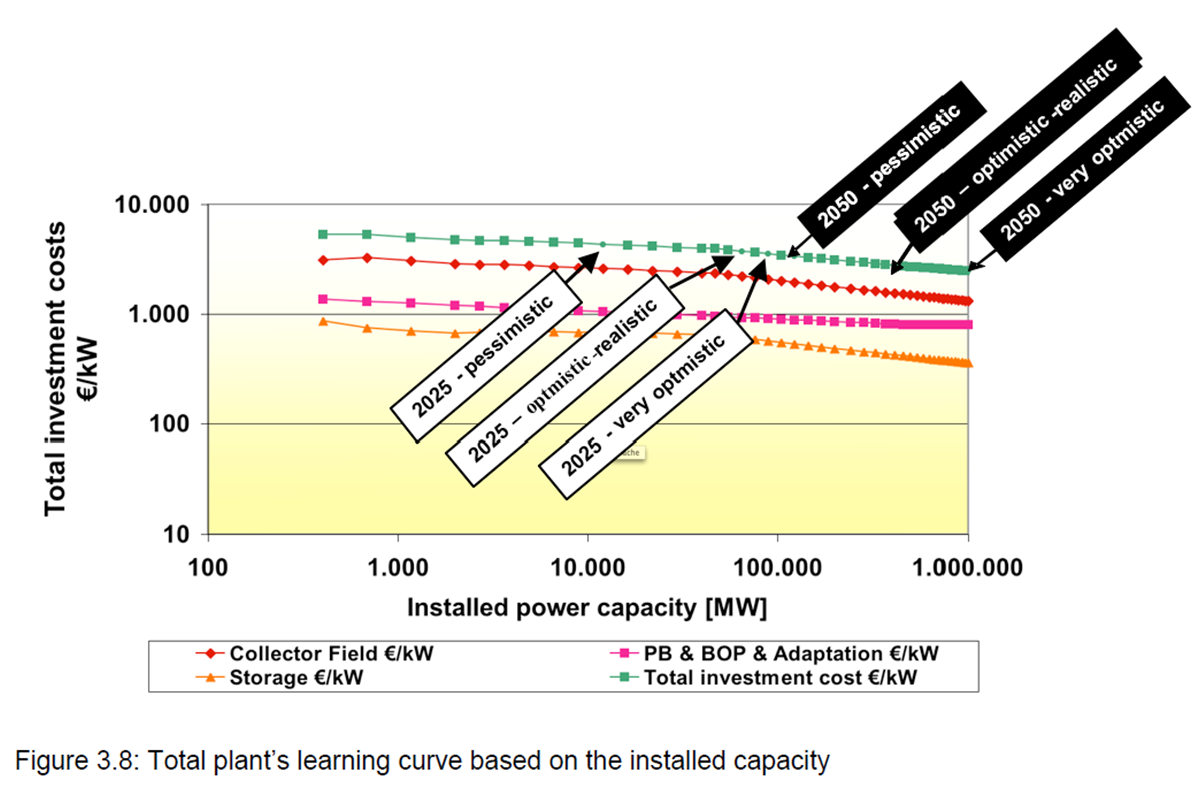
\includegraphics[width=0.9\textwidth]{kostenentwicklung2.png}
	\caption{Kostenentwicklung/Lernkurven basierend auf der installierten Kapazität}
	\label{fig:kostenentwicklung2}
\end{figure}

Die Technology Roadmap der IEA~\cite{iea2010} erwartet eine Reduktion der Kosten bis 2020 zwischen 17\,\% und 40\,\%. Abbildung~\ref{fig:kostenentwicklung1} zeigt die Kostenentwicklung eines Parabolrinnenkraftwerks bis 2017 basierend auf den Ergebnissen eines Kostenmodells auf Grundlage eines 100MW-Referenzkraftwerks in Queensland.
Für Solarturmkraftwerke wird eine Reduktion der Gesamtkosten um etwa 28\,\% bis 2020 erwartet.

Zusätzlich zu diesen Kostenprognosen basierend auf Modellrechnungen gibt es Schätzungen für die allgemeine Lernrate für CSP, also die Reduktion der Kosten je Verdopplung der installierten Kapazität. In Abbildung~\ref{fig:kostenentwicklung2} sind verschiedene Lernkurven dargestellt, basierend auf unterschiedlichen Referenzszenarien~\cite{viebahn2008}. Lernraten von 8-10\,\% werden als konservativ-realistisch angesehen.

Vorsichtige Schätzungen der Stromentstehungskosten (\emph{Levelised Cost of Electricity}, LCOE) liegen derzeit bei 0,20 bis 0,33\,USD/kWh für Parabolrinnen- und zwischen $0,16$ und $0,27$\,USD/kWh für Solarturmkraftwerke. Dies ist im Vergleich mit anderen Techniken ein hoher Wert. Bis 2020 wird je nach Szenario mit einer Reduktion der Stromentstehungskosten auf wettbewerbsfähigere Werte zwischen 0,08 bis 0,16\,USD/kWh gerechnet.\cite{irena2012}

